\newpage
\section{Numerical Sequences and Series}
\subsection{Sequences}
We begin by formally defining a sequence.
\begin{ndef}{: Sequences}{}
    Let $X$ be a metric space. A \textbf{sequence} is a function $f: \NN \mapsto X$. We can denote a term in the sequence as $f(n) = x_n$, or the entire sequence as $\set{x_n}_{n=1}^\infty$, $\set{x_n}$, $(x_n)$, or $\set{x_1, x_2, x_3 \ldots}$. 
\end{ndef}
\noindent We now discuss the notion of convergence of a sequence. Intuitively, we can equate convergence with the notion of points getting closer together.
\begin{definition}{Convergence of Sequences}{3.1}
    A sequence $\set{p_n}_{n=1}^\infty$ convergence to $p \in X$ if for all $\e > 0$, there exists $N \in \NN$ such that $n \geq N$ implies $d(p_n, p) < \e$. In this case, we say that $\set{p_n}$ converges to $p$, or that $p$ is the limit of $\set{p_n}$, and denote this as $p_n \rightarrow p$ or $\lim_{n \rightarrow \infty} p_n = p$. If $\set{p_n}$ does not converge, we say it diverges.
\end{definition}
\noindent To phrase this definition in another way, we fix some $\e > 0$, and then we have that all points in the sequence past some $N \in \NN$ are contained in the neighbourhood $N_\e(p)$. In practice, it can be difficult to apply this definition of convergence if we don't know what the limiting $p$ is, as the definition implicitly uses the value of the limit. We will later discuss another definition of convergence (in $\RR^k$) that does not use the value of the limit.
\begin{figure}[htbp]
    \centering
    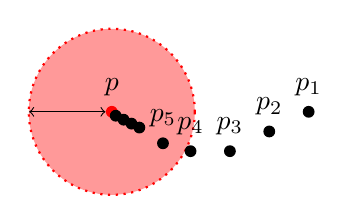
\begin{tikzpicture}[mycirc/.style={circle,fill, minimum size=0.15cm, inner sep = 0pt}]
        \draw[red, dotted, thick, fill = white!60!red] (-1, 0) circle (30pt);
        \node[mycirc, label=above:{$p$}, fill = red] at (-1, 0) {};
        \node[mycirc, label=above:{$p_1$}] at (1.5, 0) {};
        \node[mycirc, label=above:{$p_2$}] at (1, -0.25) {};
        \node[mycirc, label=above:{$p_3$}] at (0.5, -0.5) {};
        \node[mycirc, label=above:{$p_4$}] at (0, -0.5) {};
        \node[mycirc, label=above:{$p_5$}] at (-0.35, -0.4) {};
        \node[mycirc] at (-0.65, -0.2) {};
        \node[mycirc] at (-0.75, -0.15) {};
        \node[mycirc] at (-0.85, -0.1) {};
        \node[mycirc] at (-0.95, -0.05) {};
        \draw[<->] (-1.08, 0) -- (-2.05, 0);
        \node[label=above:{$\e$}] at (-1.5, -0.15) {};
    \end{tikzpicture}
    \caption{Visualization of a sequence $\set{p_n} \subset \RR^2$ converging to a point $p$. For the $\e > 0$ shown in the picture, we have that all points of the sequence past $N = 5$ lie in the open disk of radius $\e$ around $p$.}
    \label{fig15}
\end{figure}

\noindent As a remark, consider that convergence can depend on our choice of metric space; for example, $\set{\frac{1}{n}}$ as a sequence in $\RR$ converges to $0$, but the same sequence in the strictly positive reals ($\RR^+ = \set{x \in \RR: x > 0}$) does not converge.

\stepcounter{rudin}
\begin{theorem}{}{3.3}
    Suppose $\set{s_n}, \set{t_n}$ are complex sequences that converge, with $\liminfi s_n \rightarrow s$ and $\liminfi t_n \rightarrow t$. Then:
\end{theorem}
\subsection{Subsequences}
\subsection{Cauchy Sequences and Completeness}
\subsection{Limsup and Liminf}
\subsection{Series}
\subsection{The Harmonic Series and Euler's Number}
\subsection{Convergence Tests}
\subsection{Power Series}

